\begin{displayquote}
	\textsf{High-Performance Computing (HPC) most generally refers to the practice of aggregating computing power in a way that delivers much higher performance than one could get out of a typical desktop computer or workstation in order to solve large problems in science, engineering, or business. HPC is one of the most active research areas in Computer Science because it is strategically important to solve the very large challenge problems arising from scientific and industrial applications. The development of HPC relies on the efforts from multi-disciplines, including the computer architecture design, the parallel algorithms, and programming models, etc. This chapter gives the state-of-the-art in HPC: its history of evaluation, different computing, and parallel programming paradigms. In the final section, we discuss the critical challenges to the whole HPC community with the coming of exascale supercomputers.}
\end{displayquote}

\vspace{1in}

\section{History of HPC}

The terms \textit{high-performance computing} and \textit{supercomputing} are sometimes used interchangeably. HPC technology is implemented in a wide range of computationally intensive applications in multidisciplinary areas including biosciences, geographical data, electronic design, climate research, neuroscience, quantum mechanics, molecular modeling, nuclear fusion, etc. Supercomputers were introduced in the 1960s, and the performance of a supercomputer is measured in floating-point operations per second (FLOPS). Since the first generation of supercomputers, the Megascale was reached in the 1970s, and the Gigascale was passed in less than ten years. Finally, the Terascale was achieved in the 1990s, and the Petascale was crossed in 2008 with the installation IBM Roadrunner at Los Alamos National Laboratory in the United States. Fig. \ref{sc_evaluate} shows the Top 1 supercomputer's performance by year.

Since 1993, the TOP500 project ranks and details the 500 most powerful non-distributed computer systems in the world and publishes an updated list of the supercomputers twice a year. The project aims to provide a reliable basis for tracking and detecting trends in high-performance computing and bases rankings on HPL, a portable implementation of the high-performance LINPACK benchmark written in Fortran for distributed-memory computers. According to the newest Top500 list of June 2018, the fastest supercomputer is the Summit of the United States, which has a LINPACK benchmark score of 122.3 PFLOPS. The Sunway TaihuLight, Sierra and Tianhe-2A follow closely the Summit, with the performance respectively 93 PFLOPS, 71.6 PFLOPS, and 61.4 PFLOPS. 

\begin{figure}[htbp]
	\centering
	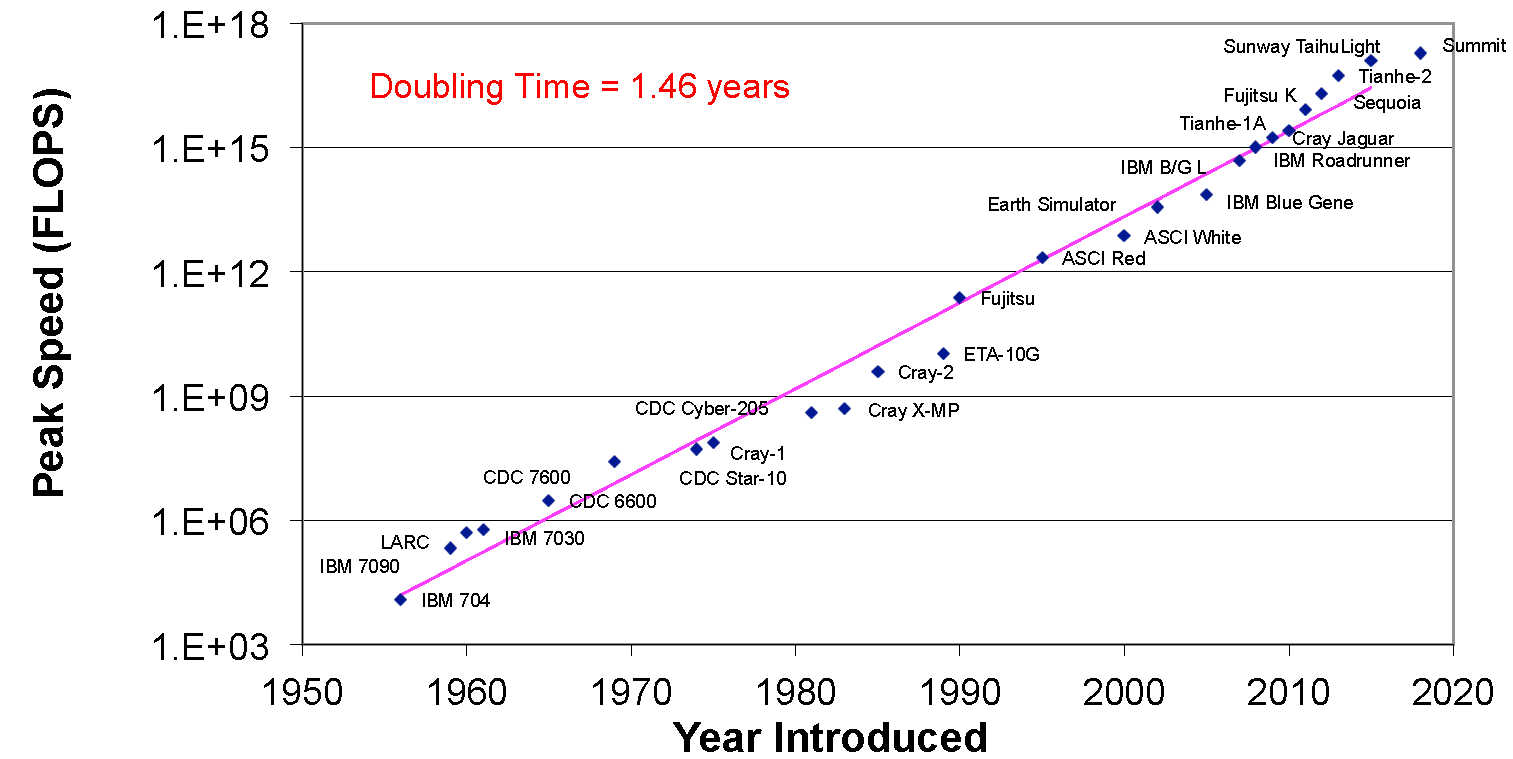
\includegraphics[width=6.3in]{fig/sc_evaluate.pdf}
	\caption{Top 1 Supercomputers' Performance by Year.}
		\label{sc_evaluate}
\end{figure}

The next barrier to overcome is the Exascale computing, which refers to computing systems capable of at least one exaFLOPS. This capacity represents a thousandfold increase over the first petascale computer which came into operation in 2008. The world first exascale supercomputer will come around 2020. China's first exascale supercomputer will enter service by 2020 according to the head of the school of computing at the National University of Defense Technology (NUDT). United States's first Exascale computer is planned to be built by 2021 at Argonne National Laboratory. The post-K announced by Japan will start the public service around 2021, and the first exascale supercomputer in Europe will appear around 2022. Exascale computing would be considered as a significant achievement in computer engineering, for it is estimated to be the order of processing power of the human brain at the neural level.

Considering the evaluation of HPC, there are always two questions proposed to the users:

\begin{itemize}
	\item How to build such powerful machines?
	\item How can the users develop applications to profit the computational capacity of supercomputers efficiently?
\end{itemize}

In order to answer these two questions above, this chapter firstly gives a glance at the modern computing architectures to build the supercomputers, and then different parallel programming models to develop the applications to benefit the whole computational power of these supercomputers.


\section{Modern Computing Architectures}

Different architectures of computing units are designed to build the supercomputers. In this section, the state-of-art of modern CPUs and accelerators are reviewed.

\subsection{CPU Architectures and Memory Access}

The \textit{Von Neumann architecture} is a computer architecture based on the description by the mathematician and physicist \textit{John von Neumann} and others in the \textit{First Draft of a Report on the EDVAC}. All the modern computing units are all envolved from this concept, which consists of five parts:

\begin{itemize}
	\item A \textit{processing unit} that contains an arithmetic logic unit and processor registers;
	\item A\textit{control unit} that contains an instruction register and program counter;
	\item \textit{Memory} that stores data and instructions;
	\item External mass \textit{storage};
	\item \textit{Input/output} mechanisms.
\end{itemize}

As shown in Fig. \ref{von-neumann}, the \textit{Von Neumann architecture} uses the shared bus between the program memory and data memory, which leads to its bottleneck. Since the single bus can only access one of the two types of memory at a time, the data transfer rate between the CPU and memory is rather low. With the increase of CPU speed and memory size,  the bottleneck has become more of a problem.

\begin{figure}[t]
	\centering
	\subfloat[Von Neumann architecture.]{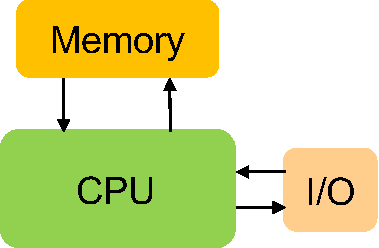
\includegraphics[width=1.8in]{fig/von-neumann.pdf}%
		\label{von-neumann}}
	\hspace{8.5pt}
	\subfloat[Harvard architecture.]{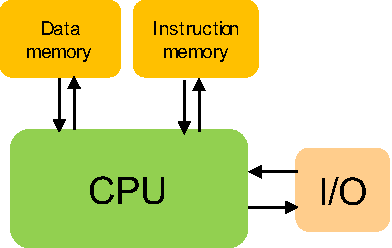
\includegraphics[width=1.8in]{fig/harvard.pdf}%
		\label{havard}}
	\hspace{8.5pt}
	\subfloat[Modified Harvard architecture.]{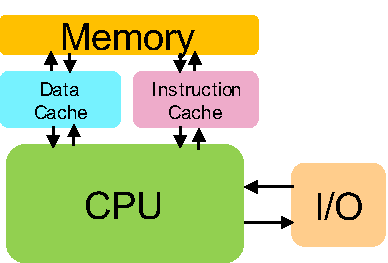
\includegraphics[width=1.8in]{fig/modified-harvard.pdf}%
	\label{modified-havard}}
	\caption{ Computer architectures.}
	\label{cpu-arch}
\end{figure}

The \textit{Harvard architecture} is another computer architecture with physically separate the storage and bus for the instructions and data. As shown in Fig. \ref{havard}, the limitation of a pure Harvard architecture is that the mechanisms must be provided to load the program to be executed into instruction memory separately and any data to be operated upon input memory. Additionally, read-only technology for the instruction memory allows the computer to begin execution of a pre-loaded program as soon as power is applied. The data memory will at this time be in an unknown state, so it is not possible to provide any kind of pre-defined data values to the program.

Today, most processors implement the separate pathways as \textit{Harvard architecture} to support the higher performance concurrent data and instruction access, meanwhile loosen the strictly separated storage between code and data. That is named as the \textit{Modified Havard architecture} (shown as Fig. \ref{modified-havard}). This model can be seen as the combination of the \textit{Von Neumann architecture} and  \textit{Harvard architecture}.

The solution is to provide a hardware pathway and machine language instructions so that the contents of the instruction memory can be read as if they were data. Initial data values can then be copied from the instruction memory into data memory when the program starts. If the data is not to be modified, it can be accessed by the running program directly from instruction memory without taking up space in the data memory.

Nowadays, most CPU has Von Neumann like unified address space and also separate instruction and data caches as well as memory protection, making them more Harvard-like, and so they could be classified more as \textit{modified Harvard architecture} even using unified address space.

\begin{figure}[htbp]
	\centering
	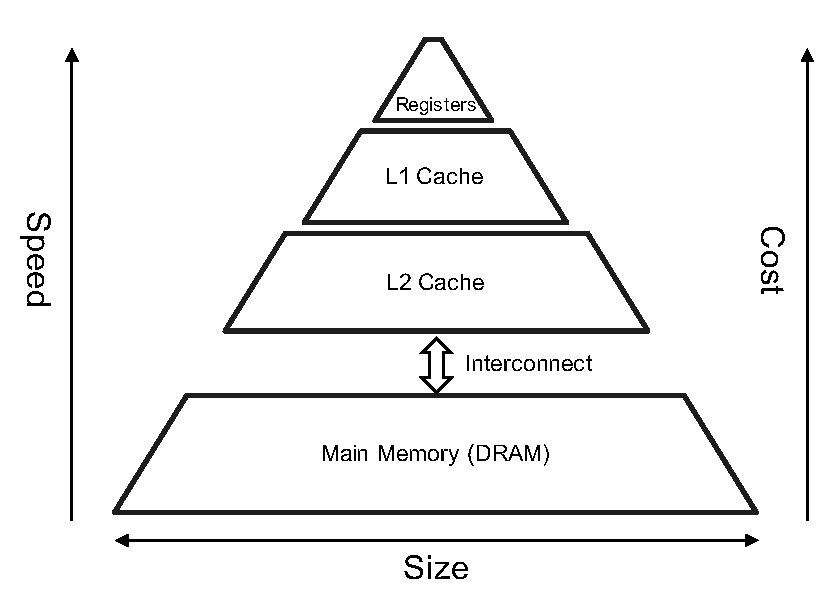
\includegraphics[width=4.6in]{fig/memory.pdf}
	\caption{Memory Hierarchy.}
	\label{fig:memory-access}
\end{figure}

The most common modification on \textit{modified Harvard architecture}  for modern CPUs is to build a memory hierarchy with a CPU cache separating instructions and data based on response time. As shown in Fig. \ref{fig:memory-access}, the top of the memory hierarchy which provides the fastest data transfer rate are the registers. Target data with arithmetic and logic operations will be temporarily held in the register to perform the computations. The number of registers is limited due to the cost. A CPU cache is a hardware cache used by CPU to reduce the average cost (time or energy) to access data from the main memory. A cache is a smaller, faster memory, closer to a processor core, which stores copies of the data from frequently used main memory locations. Most CPUs have different independent caches, including instruction and data caches, where the data cache is usually organized as a hierarchy of more cache levels. The lowest level is the main memory, which is made of Dynamic Radom-Acess Memory (DRAM) with the lowest bandwidth and the highest latency compared to registers and caches.

\subsection{Parallel Computer Memory Architectures}

The parallel computer memory architectures can be divided into shared and distributed memory types. The shared memory parallel computers vary widely, but generally have in common the ability for all processors to access all memory as global address space. Multiple processors can operate independently but share the same memory resources. Changes in a memory location effected by one processor are visible to all other processors. Historically, shared memory machines have been classified as \textit{Uniform Memory Access (UMA)} (shown as \ref{uma}) and \textit{Non-Uniform Memory Access (NUMA)} (shown as \ref{numa}), based upon memory access times. UMA is most commonly represented today by Symmetric Multiprocessor (SMP) machines with Identical processors. These processors require Equal access and access times to memory. NUMA Often made by physically linking two or more SMPs, one SMP can directly access memory of another SMP. Not all processors have equal access time to all memories, memory access across link is slower. The advantages of shared memory architectures are: 1) Global address space provides a user-friendly programming perspective to memory; 2) Data sharing between tasks is both fast and uniform due to the proximity of memory to CPUs. The disadvantages are: 1) the lack of scalability between memory and CPUs, in fact, adding more CPUs can geometrically increases traffic on the shared memory-CPU path, and for cache coherent systems, geometrically increase traffic associated with cache/memory management; 2) Programmer responsibility for synchronization constructs that ensure "correct" access of global memory. There is no way we can reach the hundreds of thousands of CPU-cores we need for today’s multi-petaflop supercomputers.

\begin{figure}[t]
	\centering
	\subfloat[Shared Memory Architecture (UMA).]{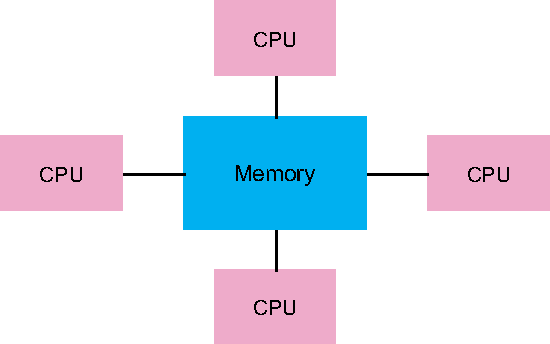
\includegraphics[width=2.6in]{fig/uma.pdf}%
		\label{uma}}
	\hspace{34.5pt}
	\subfloat[Shared Memory Architecture (NUMA)]{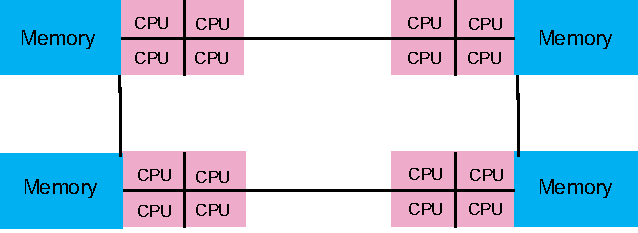
\includegraphics[width=2.6in]{fig/numa.pdf}%
		\label{numa}}
		\hspace{11.5pt}
		\subfloat[Distributed Memory Architectures.]{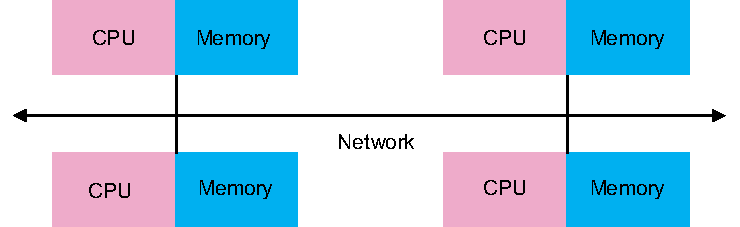
\includegraphics[width=3.1in]{fig/distributed.pdf}%
		\label{distributed}}
	\hspace{1.5pt}
	\subfloat[Distributed Shared Memory Architectures.]{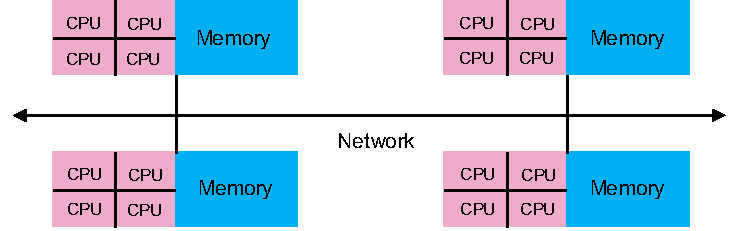
\includegraphics[width=3.1in]{fig/hybrid.pdf}%
		\label{hybrid}}
	\caption{Parallel Computer Memory Architectures.}
	\label{parallel-memory}
\end{figure}

Then the distributed-memory architecture is proposed, which takes many multicore computers and connects them together using a network, much like workers in different offices communicating by telephone. With a sufficiently fast network we can in principle extend this approach to millions of CPU-cores and beyond. As shown in Fig. \ref{distributed}, inside distributed memory system, processors have their own local memory. Memory addresses in one processor do not map to another processor, so there is no concept of global address space across all processors. Because each processor has its own local memory, it operates independently. Changes it makes to its local memory have no effect on the memory of other processors. Hence, the concept of cache coherency does not apply. When a processor needs access to data in another processor, it is usually the task of the programmer to explicitly define how and when data is communicated. Synchronization between tasks is likewise the programmer's responsibility. The advantages of distributed memory architecture are: 1) Memory is scalable with the number of processors. Increase the number of processors and the size of memory increases proportionately; 2) Each processor can rapidly access its own memory without interference and without the overhead incurred with trying to maintain global cache coherency; 3) Cost effectiveness. The disadvantages are: 1) the programmer is responsible for many of the details associated with data communication between processors; 2) It may be difficult to map existing data structures, based on global memory, to this memory organization; 3) Non-uniform memory access times - data residing on a remote node takes longer to access than node local data.

Nowadays, the largest and fastest computers in the world employ both shared and distributed memory architectures (shown as Fig. \ref{hybrid}). The shared memory component can be a shared memory machine and/or graphics processing units (GPU). The distributed memory component is the networking of multiple shared memory/GPU machines, which know only about their own memory - not the memory on another machine. Therefore, network communications are required to move data from one machine to another. Current trends seem to indicate that this type of memory architecture will continue to prevail and increase at the high end of computing for the foreseeable future.

In a word, Shared-memory systems are difficult to build but easy to use, and are ideal for laptops and desktops. Distributed-shared memory systems are easier to build but harder to use, comprising many shared-memory nodes with their own separate memory. Distributed-shared memory systems introduce much more hierachical memory and computing with multi-level of parallelism. The important advantage of distributed-shared memory architectures is increasing scalability, and the important disadvantage is increasing the complexity to program.

\subsection{Nvidia's GPGPU}

General-purpose computing on graphics processing units (GPGPU, rarely GPGP) is the use of a graphics processing unit (GPU), which typically handles computation only for computer graphics, to perform computation in applications traditionally handled by the central processing unit (CPU). GPU was first introduced as a specialized electronic circuit designed to rapidly manipulate and alter memory to accelerate the creation of images in a frame buffer intended for output to a display device. Modern GPUs are very efficient at manipulating computer graphics and image processing. Due to its special functionality, GPGPU serves as an accelerator of CPU to improve the overall performance of computers. Nowadays, it is becoming increasingly common to use GPGPU to build the supercomputers. Until now, 5 of top 10 supercomputers in the world use GPGPU.

\begin{figure}[htbp]
	\centering
	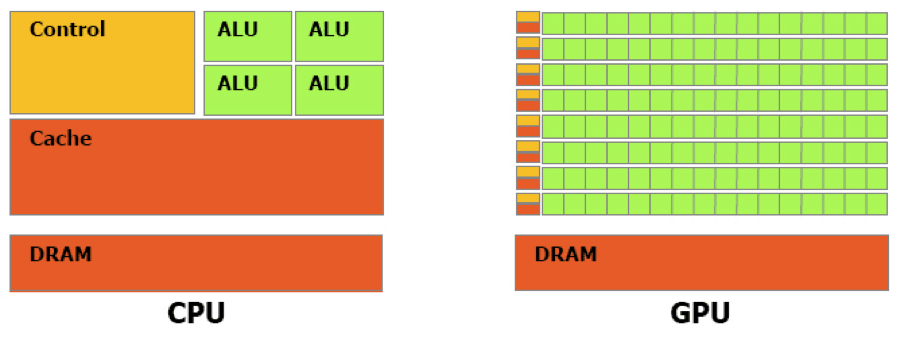
\includegraphics[width=6.in]{fig/cpu_vs_gpu.png}
	\caption{CPU vs GPU.}
	\label{cpuvsgpu}
\end{figure}

As shown in Figure \ref{cpuvsgpu}, the architectures of CPU and GPU are different: the CPU has a small number of complex cores and massive caches while the GPU has thousands of simple cores and small caches. These ALUs of GPU are simple, data-parallel, multi-threaded which offer high computing power and large memory bandwidth. In brief, graphics chips are designed for parallel computations with lots of arithmetic operations, and CPUs are for general complex applications. The host character of the CPU requires complicated cores and deep pipelines to deal with all kinds of operations. It usually runs at a higher frequency and supports branch prediction. The GPU only focuses on data-parallel image renderings thus the pipeline is shallow. The same instructions are used on large datasets in parallel with thousands of hardware cores, so the branch prediction is not necessary, and memory access latency is hidden by important arithmetic operations instead of caching. GPGPU is also regarded as a powerful backup to overcome the \textit{power wall}.

Introduced in mid-2017, the newest Tesla V100 card can deliver $7.8$ TFLOPS in double-precision floating point and $15.7$ TFLOPS for single-precision.

\subsection{Intel's Many Integrated Cores}

The performance improvement of processors comes from the increasing number of computing units within the small chip area. Thanks to advanced semiconductor processes, more transistors can be built in one shared-memory system to do multiple things at once: from the view of programmers, this can be realized in two ways: different data or tasks execute in multiple individual computing units (multi-thread) or long uniform instruction decoders (vectorization).

\begin{figure}[htbp]
	\centering
	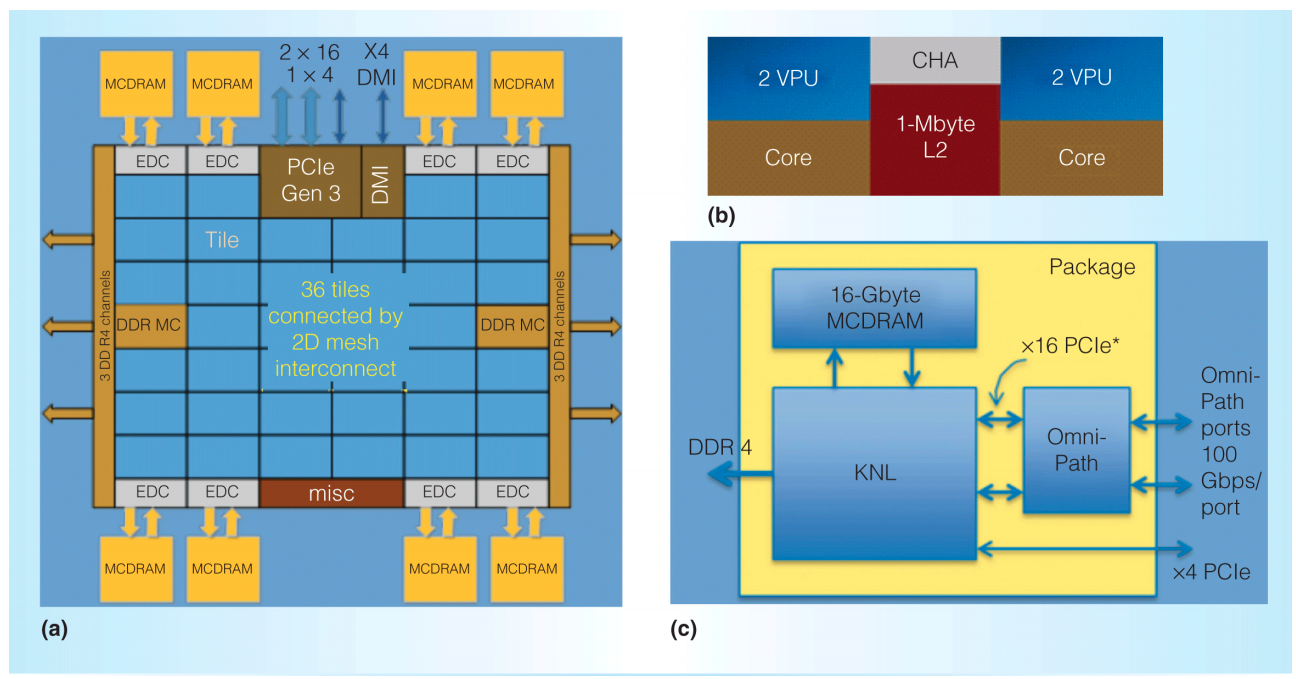
\includegraphics[width=6.2in]{fig/KNL1.png}
	\caption{The organization of a Knights Landing processor.}
	\label{knl1}
\end{figure}

Intel officially first revealed the latest MIC codenamed Knights Landing (KNL) in 2013. Being available as a coprocessor like previous boards, KNL can also serve as a self-boot MIC processor that is binary compatible with standard CPUs and boot
standard OS. These second generation chips could be used as a standalone CPU, rather than just as an add-in card. Another key feature is the on-card high-bandwidth memory (HBM) which provides high bandwidth and large capacity to run large HPC workloads. Memory bandwidth is one of the common performance bottlenecks for computational applications due to the memory wall. KNL implements a two-level memory system to address this issue. It shares application areas with GPUs. The main difference between Xeon Phi and a GPGPU like Nvidia Tesla is that Xeon Phi, with an x86-compatible core, can, with less modification, run software that was originally targeted at a standard x86 CPU.

\subsection{Others}

There are also processors designed for supercomputing, for example, the SW26010 and Matrix-2000. The SW26010 is a 260-core manycore processor \cite{fu2016sunway} designed by the National High-Performance Integrated Circuit Design Center in Shanghai. It implements the Sunway architecture, a 64-bit reduced instruction set computing (RISC) architecture designed by China. The SW26010 has four clusters of 64 Compute-Processing Elements (CPEs) which are arranged in an eight-by-eight array. The CPEs support SIMD instructions and are capable of performing eight double-precision floating-point operations per cycle. Each cluster is accompanied by a more conventional general-purpose core called the Management Processing Element (MPE) that provides supervisory functions. Each cluster has its own dedicated DDR3 SDRAM controller and a memory bank with its own address space. The processor runs at a clock speed of 1.45.

Matrix-2000 \cite{zhang2018mocl} is a 64-bit 128-core many-core processor designed by NUDT and introduced in 2017. This chip was designed exclusively as an accelerator for China's Tianhe-2 supercomputer in order to upgrade and replace the aging Intel's Knights Corner accelerators. The Matrix-2000 features 128 RISC cores operating at 1.2 GHz achieving 2.46/4.92 TFLOPS (DP/SP) with a peak power dissipation of 240W. The Matrix-2000 consists of 128 cores, eight DDR4 memory channels, and x16 PCIe lanes. The chip consists of four supernodes (SN) consisting of 32 cores each operating at 1.2 GHz with a peak power dissipation of 240 Watts.

\section{Parallel Programming Model}

After the introduction of hardware architectures, we will present the different parallel programming models on top of them in this section.

\subsection{OpenMP}
OpenMP (Open Multi-Processing) \cite{dagum1998openmp} is an application programming interface (API) that supports multi-platform shared memory parallel programming in C, C++, and Fortran. OpenMP supports most platforms, instruction set architectures, and operating systems. It consists of a set of compiler directives, library routines, and environment variables. OpenMP provides the capability to incrementally parallelize a serial program with by inserting the specific directives. These directives can be ignored by the compiler, and the application can be executed in a sequential way when target machines do not support OpenMP. OpenMP is designed for multi-processor/core, shared memory machines. The underlying architecture can be shared memory UMA or NUMA. OpenMP programs accomplish parallelism exclusively through the use of threads.

\begin{figure}[htbp]
	\centering
	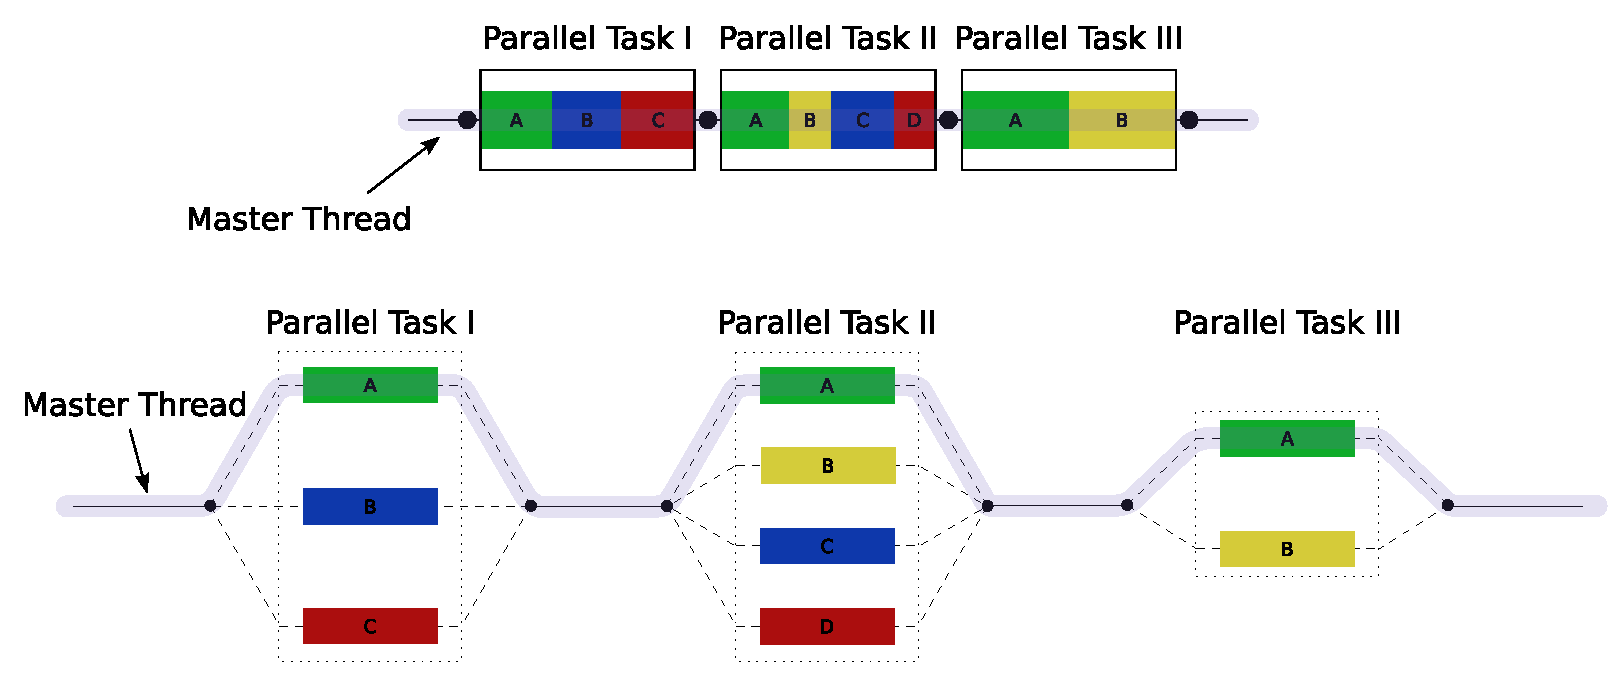
\includegraphics[width=6.3in]{fig/Fork_join.pdf}
	\caption{OpenMP \textbf{fork-join} Model.}
	\label{openmp_fork_join}
\end{figure}

As shown in Fig. \ref{openmp_fork_join}, OpenMP uses the \textbf{fork-join} model to support parallel execution. All OpenMP programs begin with a single process which executes utils sequentially the first parallel region construct is encountered.  Then this thread creates a team of parallel threads and distributes the workload to them in order to have them work simultaneously. When the team threads complete the statements in the parallel region construct, they synchronize and terminate, leaving only the master thread. The new released OpenMP begins to support task scheduling strategies, the SIMD directives for high-level vectorization and the \textit{offload} directives for heterogeneous systems.

\subsection{CUDA}

CUDA (Compute Unified Device Architecture) \cite{nvidia2011nvidia} is a parallel programming platform and application programming interface model created by Nvidia. It allows software developers and software engineers to use a CUDA-enabled GPU for general purpose processing. The CUDA software layer gives direct access to GPU's virtual instruction set de parallel computational elements, for the execution of compute kernels. The CUDA platform is designed to work with programming languages such as C, C++, and Fortran. This accessibility makes it easier for specialists in parallel programming to use GPU resources. CUDA supports programming frameworks such as OpenACC and OpenCL.

\begin{figure}[htbp]
	\centering
	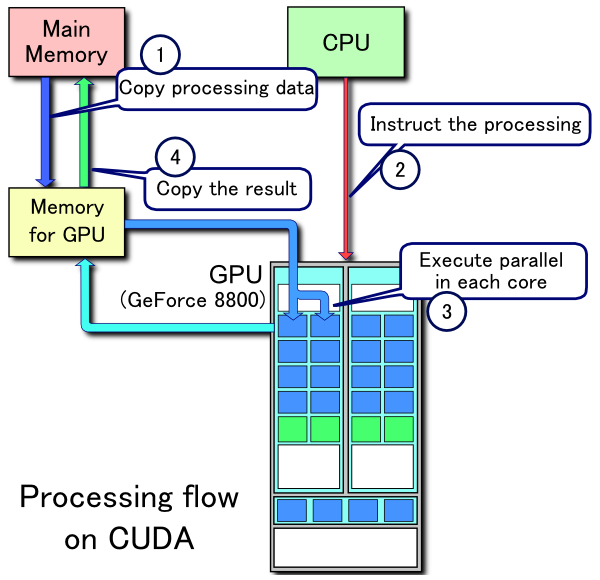
\includegraphics[width=4.2in]{fig/CUDA.png}
	\caption{Processing flow on CUDA.}
	\label{cuda_flow}
\end{figure}

\subsection{Message Passing Interface}

MPI (Message Passing Interface) \cite{gropp1999using} is a standardized and portable message-passing standard designed by a group of researchers from academia and industry to support a wide variety of parallel computing architectures. MPI provides a simple-to-use portable interface for the basic user, yet one powerful enough to allow programmers to use the high-performance message passing operations available on advanced machines. Most MPI implementations consist of a specific set of routines directly callable from C, C++, Fortran and any language able to interface with such libraries. The MPI interface is meant to provide essential virtual topology, synchronization, and communication functionality between a set of processes (that have been mapped to nodes/servers/computer instances) in a language-independent way, with language-specific syntax (bindings), plus a few language-specific features. 

\begin{figure}[htbp]
	\centering
	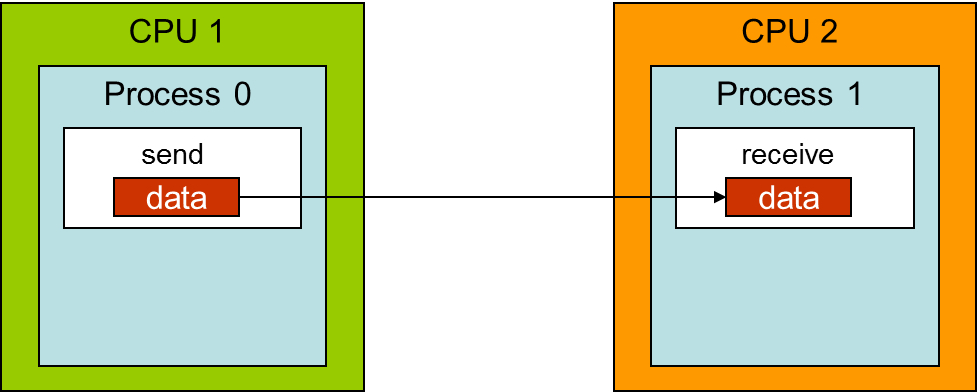
\includegraphics[width=5.4in]{fig/mpi_send_recv.jpg}
	\caption{MPI send and receive Model.}
	\label{mpi_model}
\end{figure}

MPI library functions include, but are not limited to, basic point-to-point send/receive operations, collective functions involving communication among all processes, synchronizing nodes (barrier operation), the one-sided communication, dynamic process management, I/O and so on. Point-to-point operations support both the communication in both synchronous and asynchronous ways. In modern computing platform with multiple shared-memory nodes, the shared memory programming models such as OpenMP and message passing programming such as MPI can be considered as complementary programming approaches, and can occasionally be used together in a hybrid way.

\subsection{Partitioned Global Address Space}

In computer science, a partitioned global address space (PGAS) is a parallel programming model. It assumes a global memory address space that is logically partitioned and a portion of it is local to each process, thread, or processing element. The novelty of PGAS is that the portions of the shared memory space may have an affinity for a particular process, thereby exploiting locality of reference. There are different implementation based on PGAS model, such as Unified Parallel C, Coarray Fortran, Split-C, Chapel, X10, UPC++, DASH, XcalableMP, etc. PGAS attempts to combine the advantages of an SPMD programming style for distributed memory systems (as employed by MPI) with the data referencing semantics of shared memory systems. This is more realistic than the traditional shared memory approach of one flat address space because hardware-specific data locality can be modeled in the partitioning of the address space.

\subsubsection{XcalableMP}

XcalableMP \cite{lee2010implementation} is a language extension of C and Fortran for parallel programming on distributed memory systems that help users to reduce those programming efforts. XcalableMP provides two programming models. The first one is the global view model, which supports typical parallelization based on the data and task parallel paradigm, and enables parallelizing the original sequential code using minimal modification with simple, OpenMP-like directives. The other one is the local view model, which allows using CAF-like expressions to describe inter-node communication. Users can even use MPI and OpenMP explicitly in our language to optimize performance explicitly.

\subsection{Task/Graph Based Parallel Programming}

With the increase of the complexity of applications on the supercomputers, it is more and more difficult for the developers to maintain the parallel codes on the modern computing architectures. The task/graph based parallel programming models are proposed to express the task parallelism and data dependencies of complex codes. In this section, we list several well-known task/graph based parallel programming models.

\subsubsection{YML}

YML \cite{delannoyyml} allows you to transparently use one or more grid middleware to run an application. For this, the project is based on a dedicated language named YvetteML. YML can describe a complex parallel application regardless of the execution platform. The YvetteML language is used to express the task graph of the application. The nodes of the graph are the tasks described by components, and the edges correspond to dependencies or communications. The components are written in XML. Each component implementation can contain C ++, XMP-C, XMP-FORTRAN or other code. Each component implementation can be expressed with finer grain parallelism.

\subsubsection{StarPU}

StarPU\footnote{http://starpu.gforge.inria.fr} \cite{augonnet2011starpu} is a task programming library for hybrid architectures. The application provides algorithms and constraints:
\begin{itemize}
	\item CPU/GPU implementations of tasks;
	\item A graph of tasks, using either the StarPU's high-level GCC plugin pragmas, StarPU's rich C/C++ API, or OpenMP pragmas.
\end{itemize}

StarPU handles run-time concerns:
\begin{itemize}
	\item Task dependencies;
	\item Optimized heterogeneous scheduling;
	\item Optimized data transfers/replication between main memory and discrete memories;
	\item Optimized cluster communications.
\end{itemize}
\subsubsection{Swift}

Swift\footnote{http://swift-lang.org/main/index.php} \cite{wilde2011swift} is a data-flow oriented coarse-grained scripting language that supports dataset typing and mapping, dataset iteration, conditional branching, and procedural composition. Swift programs (or workflows) are written in a language called Swift. Swift scripts are primarily concerned with processing (possibly large) collections of data files, by invoking programs to do that processing. Swift handles execution of such programs on remote sites by choosing sites, handling the staging of input and output files to and from the chosen sites and remote execution of programs.

\subsubsection{Legion}

Legion\footnote{http://legion.stanford.edu} \cite{grimshaw1994synopsis} is a data-centric parallel programming system for writing portable high performance programs targeted at distributed heterogeneous architectures. Legion presents abstractions which allow programmers to describe properties of program data (e.g., independence, locality). By making the Legion programming system aware of the structure of program data, it can automate many of the tedious tasks programmers currently face, including correctly extracting task- and data-level parallelism and moving data around complex memory hierarchies. A novel mapping interface provides explicit programmer controlled placement of data in the memory hierarchy and assignment of tasks to processors in a way that is orthogonal to correctness, thereby enabling easy porting and tuning of Legion applications to new architectures.


\section{Exascale Challenges of Supercomputers}

 (\textcolor{red}{This section need be rewritten})
 
According to Moore's law, the number of transistors per integrated circuit doubles every $2$ years, which means that the size of the transistor is reduced to half. Moore's law is found to be acceptable utils 2002. Since then, the overheating introduced by higher frequency reaches the limit of air cooling. This is the famous \textit{power wall}. The modern architectures with multiple processors on-chip, lower operating frequency and hierarchical architectures come, such as the GPU, MIC, SW26010, and Matrix-2000.

\begin{figure}[htbp]
	\centering
	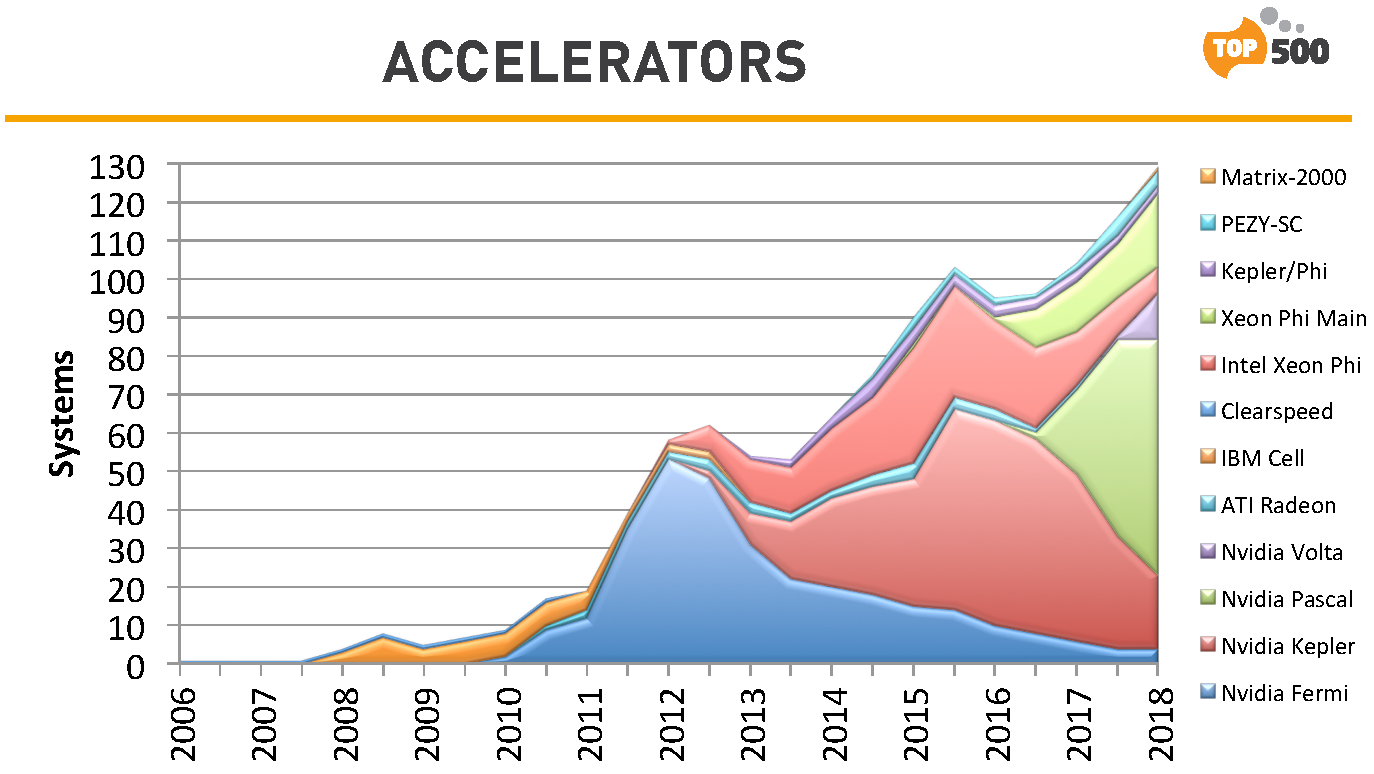
\includegraphics[width=6.6in]{fig/top500.pdf}
	\caption{Top 1 Supercomputers' Performance by Year.}
	\label{top500-acc}
\end{figure}

\begin{itemize}
	\item Highly hierarchical architectures of computing and memory;
	\item Increasing levels and degree of parallelism;
	\item Heterogeneity of computing, memory, and scalability;
	\item Requirement of parallel programming:
	\begin{itemize}
		\item multi-grain;
		\item multi-level memory;
		\item reducing synchronizations and promoting asynchronicity;
		\item multi-level scheduling strategies.
	\end{itemize}
\end{itemize}


\clearemptydoublepage